\section*{Question 2}
\subsection{Équations du mouvement}
Intéressons nous maintenant au cas où les deux corps sont de masse similaire. L'Hamiltonien du système doit bien entendu être redéfini, il est maintenant donné par 

$$\Ha(p_1,p_2,q_1,q_2) = \frac{1}{2} (\frac{1}{m_1} p_1^T p_1 + \frac{1}{m_2} p_2^T p_2) - G \frac{m_1 m_2}{||q_1- q_2||_2} $$

où $G$ représente la constante gravitationnelle et $m_i$ ma masse du corps $i$. On garde les mêmes conventions qu'à la question 1, c'est à dire que 
 $$q =
\begin{pmatrix}
  q_1\\
  q_2
\end{pmatrix},$$

$$p =
\begin{pmatrix}
  p_1\\
  p_2
\end{pmatrix},$$

avec $p_1$, $p_2$, $q_1$ et $q_2$ qui sont de la forme 
$$q_1 =
\begin{pmatrix}
  q_{11}\\
  q_{12}
\end{pmatrix},
q_2 =
\begin{pmatrix}
  q_{21}\\
  q_{22}
\end{pmatrix}$$
$$p_1 =
\begin{pmatrix}
  p_{11}\\
  p_{12}
\end{pmatrix},
p_2 =
\begin{pmatrix}
  p_{21}\\
  p_{22}
\end{pmatrix}
$$
 et
$f_1(q,p)$ et $f_2(q,p)$ sont tels que
\begin{align*}
  \dot{q} & = f_1(p,q)\\
  \dot{p} & = f_2(p,q).
\end{align*}

On calcule, en se rappelant des résultats de la question 1 mais en n'oubliant cependant pas d'inclure les masses, 
 
\begin{align*}
 f_{1,i}(q,p) &= m_i \fpart{\Ha(p,q)}{p_i} \\	
  f_1(p) & =
  \begin{pmatrix}
    m_1\frac{p_1}{m_1}\\
    m_2\frac{p_2}{m_2}
  \end{pmatrix}\\
  & = p\\
%	
 f_{2,i}(q,p) &= -\frac{1}{m_i}\fpart{\Ha(p,q)}{q_i} \\
  f_2(q) & = Gm_1m_2
  \begin{pmatrix}
    \frac{-(q_1-q_2)}{m_1\|q_1-q_2\|_2^3}\\
    \frac{(q_1-q_2)}{m_2\|q_1-q_2\|_2^3}
  \end{pmatrix}\\
  & = G
  \begin{pmatrix}
    \frac{-m_2 (q_1-q_2)}{\|q_1-q_2\|_2^3}\\
    \frac{m_1 (q_1-q_2)}{\|q_1-q_2\|_2^3}
  \end{pmatrix}.
\end{align*}

On obtient finalement notre système de 8 équations différentielles à 8 variables, qu'on va résoudre numériquement, comme dans la question 1, aux moyens des méthodes d'Euler explicite et symplectiques.\\
On choisit comme condition initiales : 
$$
q_1 = \begin{pmatrix}
0.4\\
0
\end{pmatrix},
q_2 = \begin{pmatrix}
0\\
0
\end{pmatrix},
p_1 = \begin{pmatrix}
0\\
2
\end{pmatrix},
p_2 = \begin{pmatrix}
0\\
-2
\end{pmatrix},
$$

\subsection{Analyse de la solution}

Commençons par calculer la jacobienne du système. Pour cela, calculons $\fpart{f_2}{q}$ :
$$
\begin{pmatrix}
\frac{Gm_2(2(q_{11}-q_{21})^2 - (q_{12} - q_{22})^2)}{||q||^5_2} & \frac{3Gm_2(q_{11}-q_{21})(q_{12} - q_{22}))}{||q||^5_2} & \frac{Gm_2(-2(q_{11}-q_{21})^2 + (q_{12} - q_{22})^2)}{||q||^5_2} & \frac{3Gm_2(q_{11}-q_{21})(q_{12} - q_{22}))}{||q||^5_2} \\
\frac{3Gm_2(q_{11}-q_{21})(q_{12} - q_{22}))}{||q||^5_2} & \frac{Gm_2(2(q_{12}-q_{21})^2 - (q_{11} - q_{21})^2)}{||q||^5_2} & \frac{3Gm_2(q_{11}-q_{21})(q_{12} - q_{22}))}{||q||^5_2} & \frac{Gm_2(-2(q_{12}-q_{22})^2 + (q_{11} - q_{21})^2)}{||q||^5_2} \\
\frac{-Gm_1(2(q_{11}-q_{21})^2 - (q_{12} - q_{22})^2)}{||q||^5_2} & \frac{-3Gm_1(q_{11}-q_{21})(q_{12} - q_{22}))}{||q||^5_2} & \frac{-Gm_1(-2(q_{11}-q_{21})^2 + (q_{12} - q_{22})^2)}{||q||^5_2} & \frac{-3Gm_1(q_{11}-q_{21})(q_{12} - q_{22}))}{||q||^5_2} \\
\frac{-3Gm_1(q_{11}-q_{21})(q_{12} - q_{22}))}{||q||^5_2} & \frac{-Gm_1(2(q_{12}-q_{21})^2 - (q_{11} - q_{21})^2)}{||q||^5_2} & \frac{-3Gm_1(q_{11}-q_{21})(q_{12} - q_{22}))}{||q||^5_2} & \frac{-Gm_1(-2(q_{12}-q_{22})^2 + (q_{11} - q_{21})^2)}{||q||^5_2} \\
\end{pmatrix}
$$

La jacobienne est donnée par : 
\begin{equation}
J(q,p) = 
\begin{pmatrix}
0 & I\\
\fpart{f_2}{q} & 0
\end{pmatrix}.
\end{equation}
Si on évalue $J(q,p)$ aux conditions initiales et qu'on calcul ses valeurs propres, on obtient : 
$$
\begin{pmatrix}
20.0431    \\
-20.0431   \\
-0.0000 +14.1726i \\
-0.0000 -14.1726i  \\
-0.0000          \\
-0.0000          \\
0.0000          \\
0.0000 
\end{pmatrix}
$$
On en conclut que le système n'est pas stable.\\

Intéressons nous maintenant aux résultats obtenus. 

	Comme l'illustre le graphe \ref{fig:q2_explicite_q}, dans le cas de la méthode d'euler explicite, les trajectoires tendent à s'éloigner au fil du temps. Ce qui est assez cohérent avec le graphe de la vitesse \ref{fig:q2_explicite_p}. En effet, sur ce dernier on constate que la vitesse augmente peu à peu, on saute de solution en solution, et donc forcément les corps peuvent parcourir une plus grande distance dans le même intervalle de temps, ce qui explique le graphe \ref{fig:q2_explicite_q}. L'énergie quant à elle augmente légèrement de manière globale  passant de $-2$ à $-1 \cdot 10^{-5}$ , mais par contre localement elle chute jusqu'à des $-7 \cdot 10{-5}$. 
	
	Ensuite pour Euler symplectique, on constate que les deux types renvoient les mêmes graphes tant pour p (\ref{fig:q2_symplectique1_p}, \ref{fig:q2_symplectique2_p}) que pour q (\ref{fig:q2_symplectique1_q}, \ref{fig:q2_symplectique2_q})  et $\Ha$ (\ref{fig:q2_symplectique1_H}, \ref{fig:q2_symplectique2_H}). Ce résultat, qui peut sembler surprenant de prime abord, est en fait cohérent. En effet, si on regarde de plus près on constate que dans les graphes de vitesse, cette dernière reste la même "à chaque tour", c'est à dire qu'on n'a pas d'erreur qui nous entraine vers une autre solution. Il en va de même pour la position qui, même si elle "monte" peu à peu à cause de l'interaction des deux corps, n'est en soit que la répétion d'un même mouvement. On n'a donc pas de risque de s'en aller vers l'une ou l'autre solution en fonction des variables sur lesquelles on applique euler explicite ou implicite.    



\begin{figure}
  \centering
  \begin{subfigure}[b]{0.3\textwidth}
    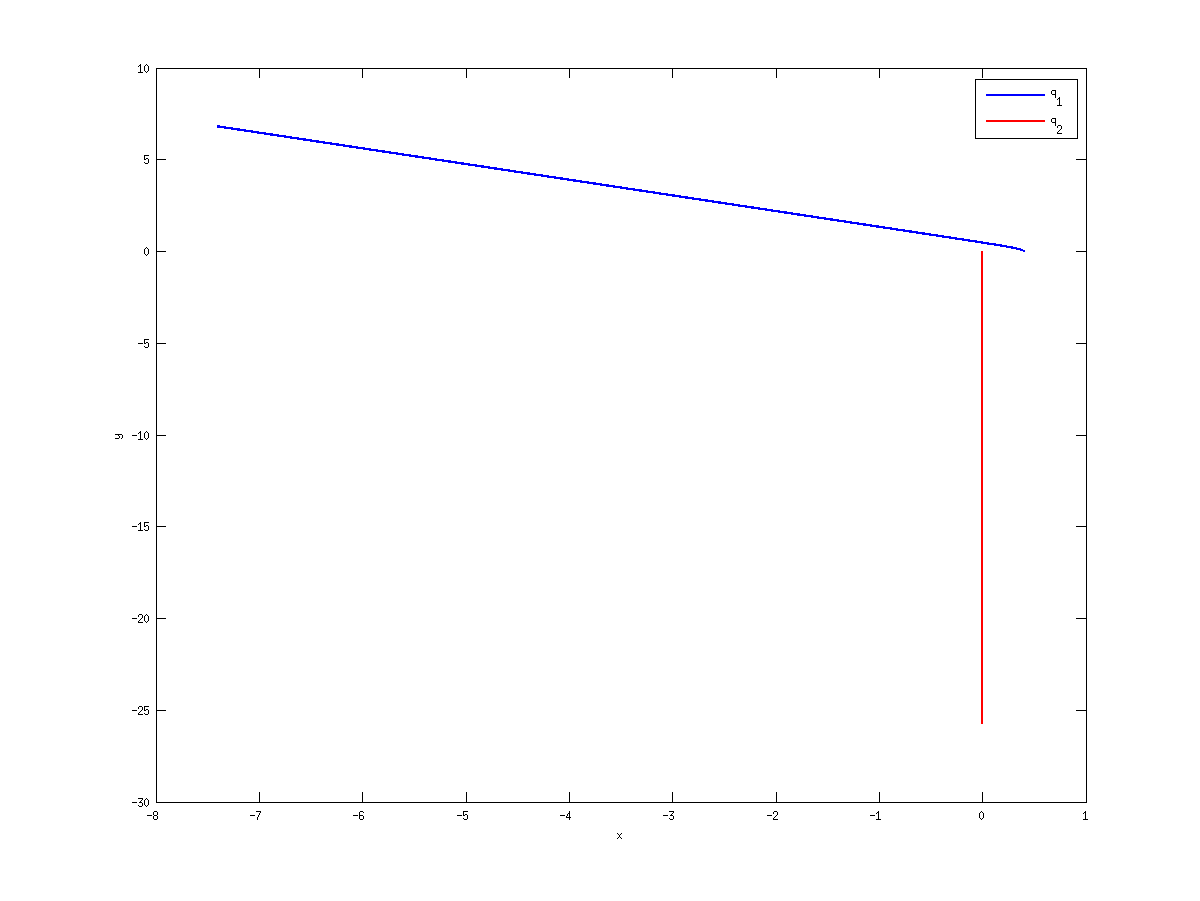
\includegraphics[width=\textwidth]{images/Q2_explicite_q.png}
    \caption{$q$ pour explicite}
    \label{fig:q2_explicite_q}
  \end{subfigure}%
  ~ %add desired spacing between images, e. g. ~, \quad, \qquad etc.
  %(or a blank line to force the subfigure onto a new line)
  \begin{subfigure}[b]{0.3\textwidth}
    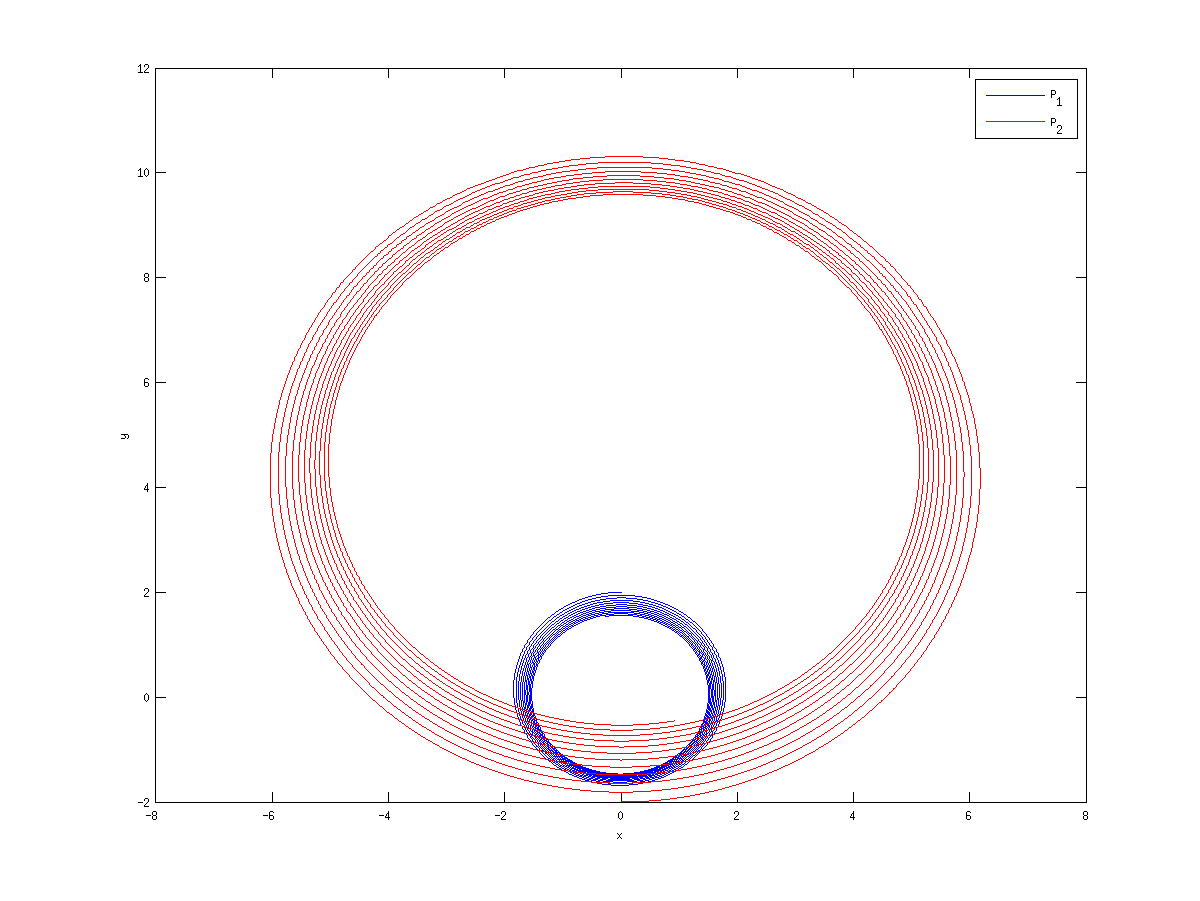
\includegraphics[width=\textwidth]{images/Q2_explicite_p.png}
    \caption{$p$ pour explicite}
    \label{fig:q2_explicite_p}
  \end{subfigure}
  ~
  \begin{subfigure}[b]{0.3\textwidth}
    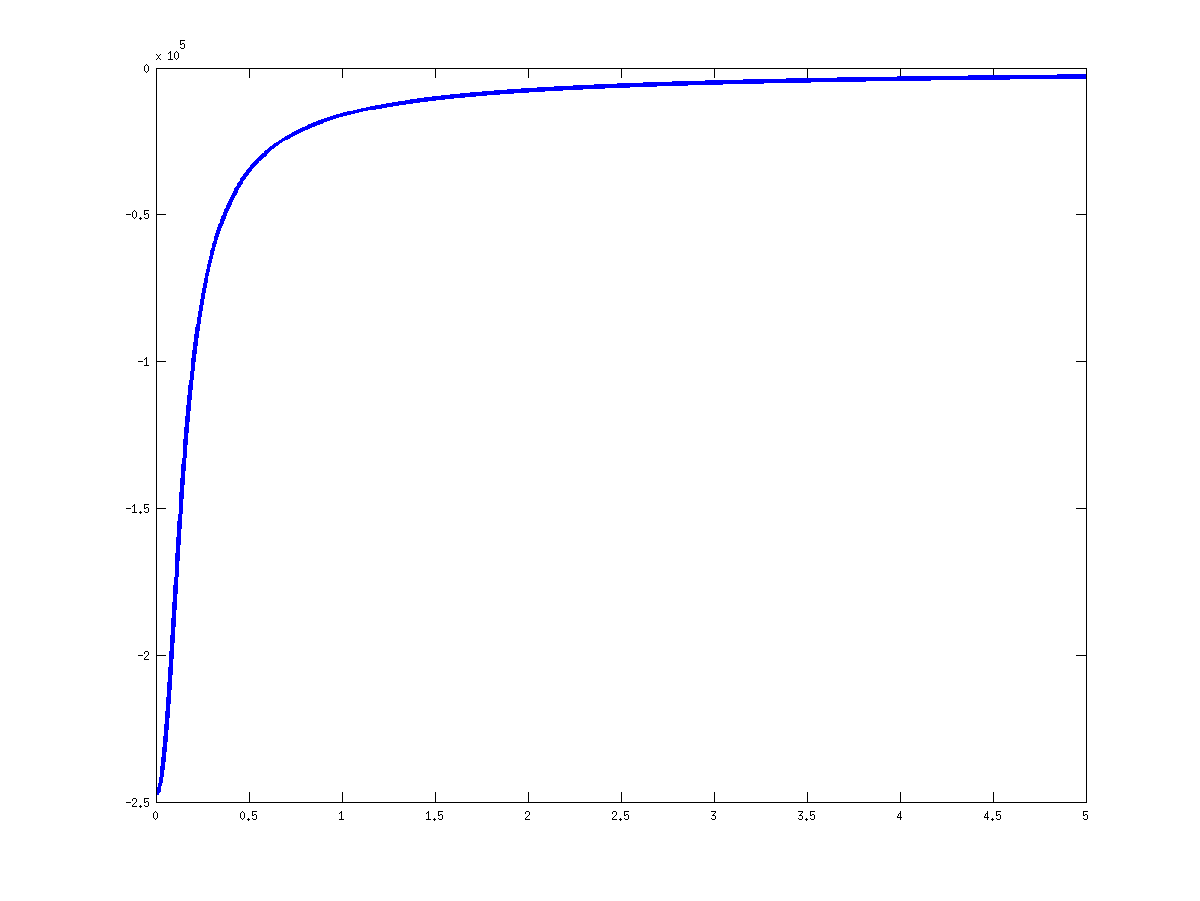
\includegraphics[width=\textwidth]{images/Q2_explicite_H.png}
    \caption{$\Ha$ pour explicite}
    \label{fig:q2_explicite_H}
  \end{subfigure}

  \begin{subfigure}[b]{0.3\textwidth}
    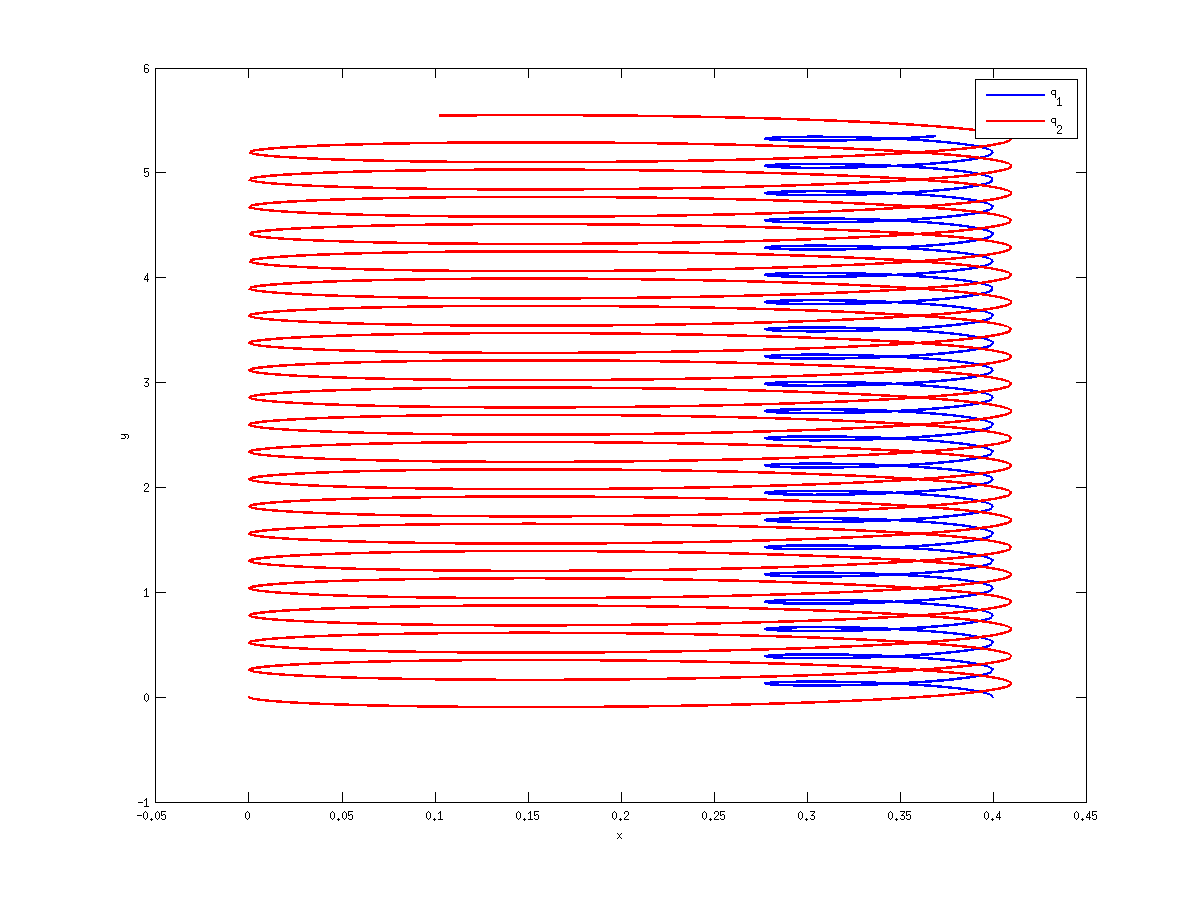
\includegraphics[width=\textwidth]{images/Q2_symplectique1_q.png}
    \caption{$q$ pour symplectique1}
    \label{fig:q2_symplectique1_q}
  \end{subfigure}%
  ~
  %(or a blank line to force the subfigure onto a new line)
  \begin{subfigure}[b]{0.3\textwidth}
    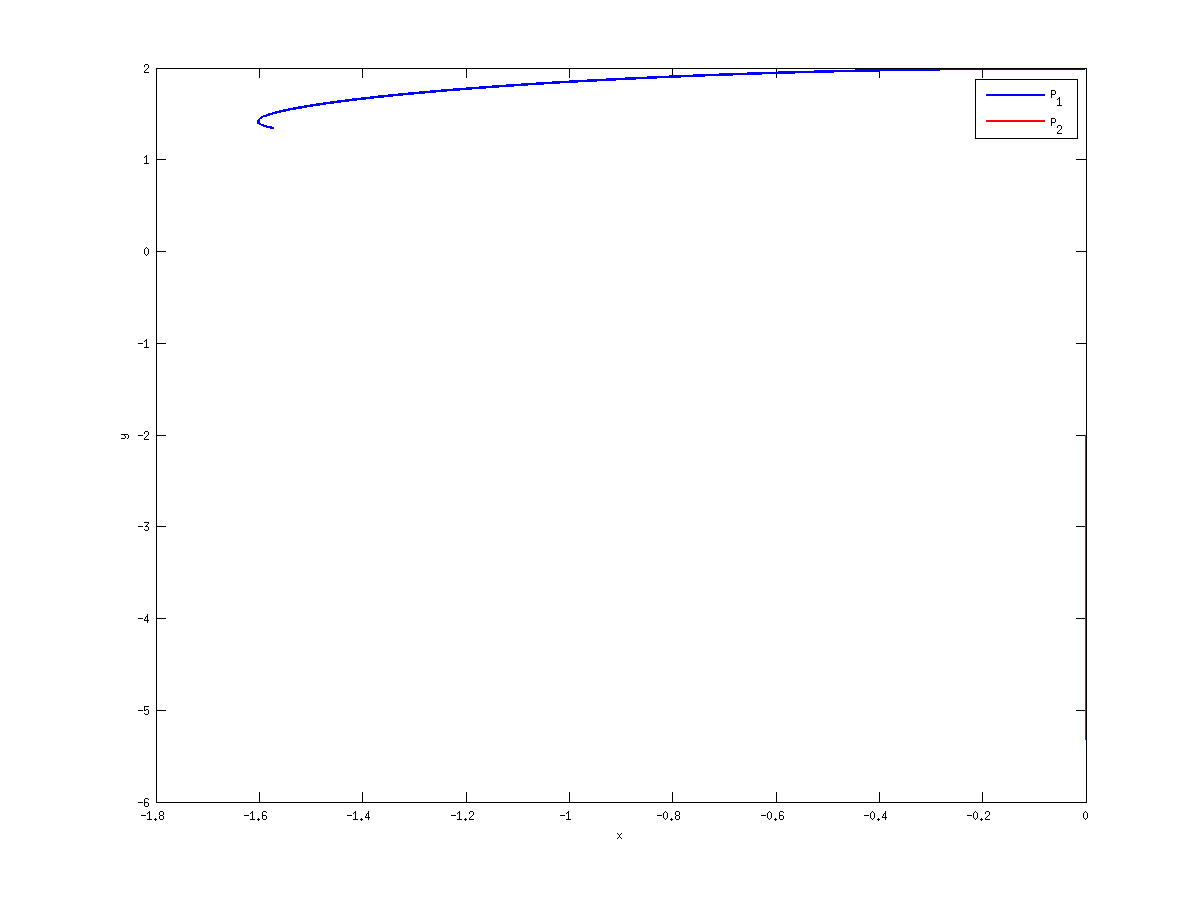
\includegraphics[width=\textwidth]{images/Q2_symplectique1_p.png}
    \caption{$p$ pour symplectique1}
    \label{fig:q2_symplectique1_p}
  \end{subfigure}
  ~
  \begin{subfigure}[b]{0.3\textwidth}
    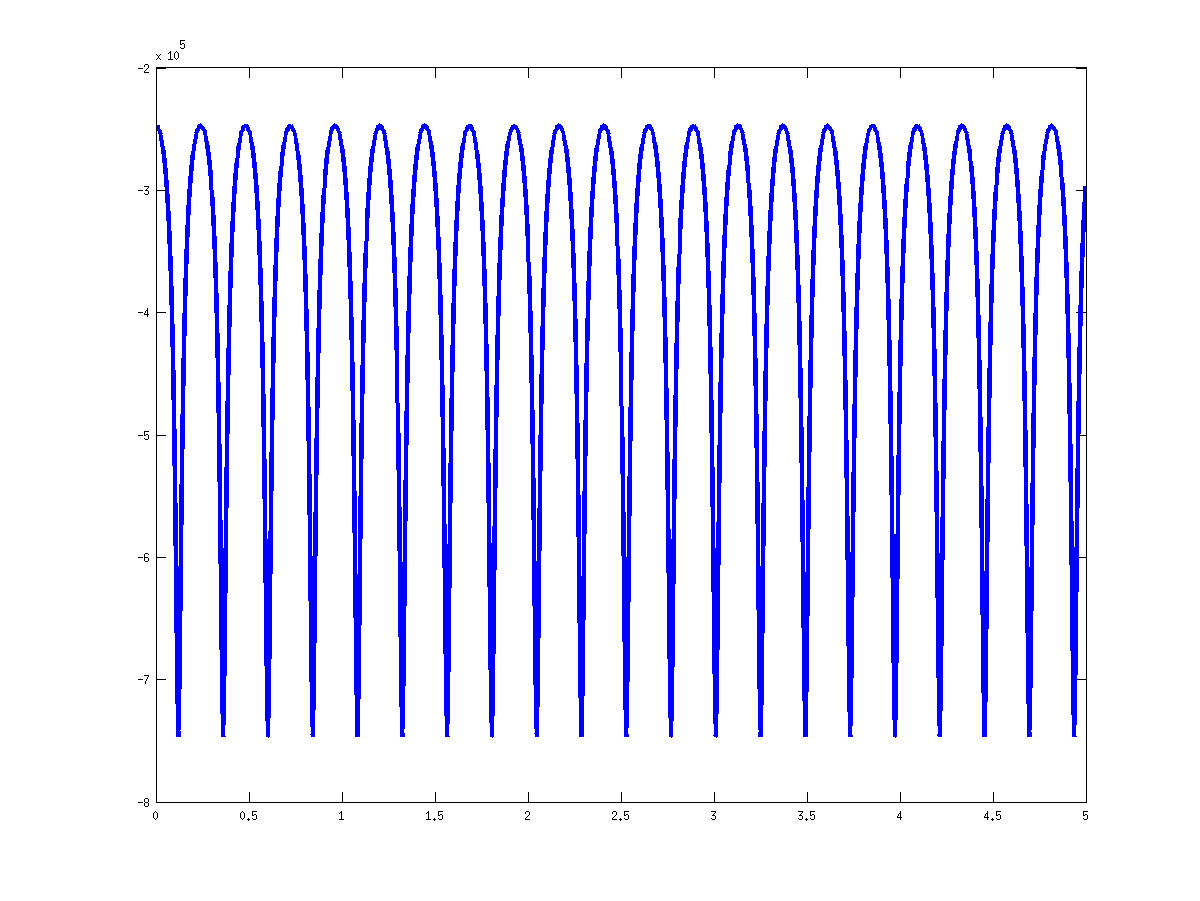
\includegraphics[width=\textwidth]{images/Q2_symplectique1_H.png}
    \caption{$\Ha$ pour symplectique1}
    \label{fig:q2_symplectique1_H}
  \end{subfigure}

  \begin{subfigure}[b]{0.3\textwidth}
    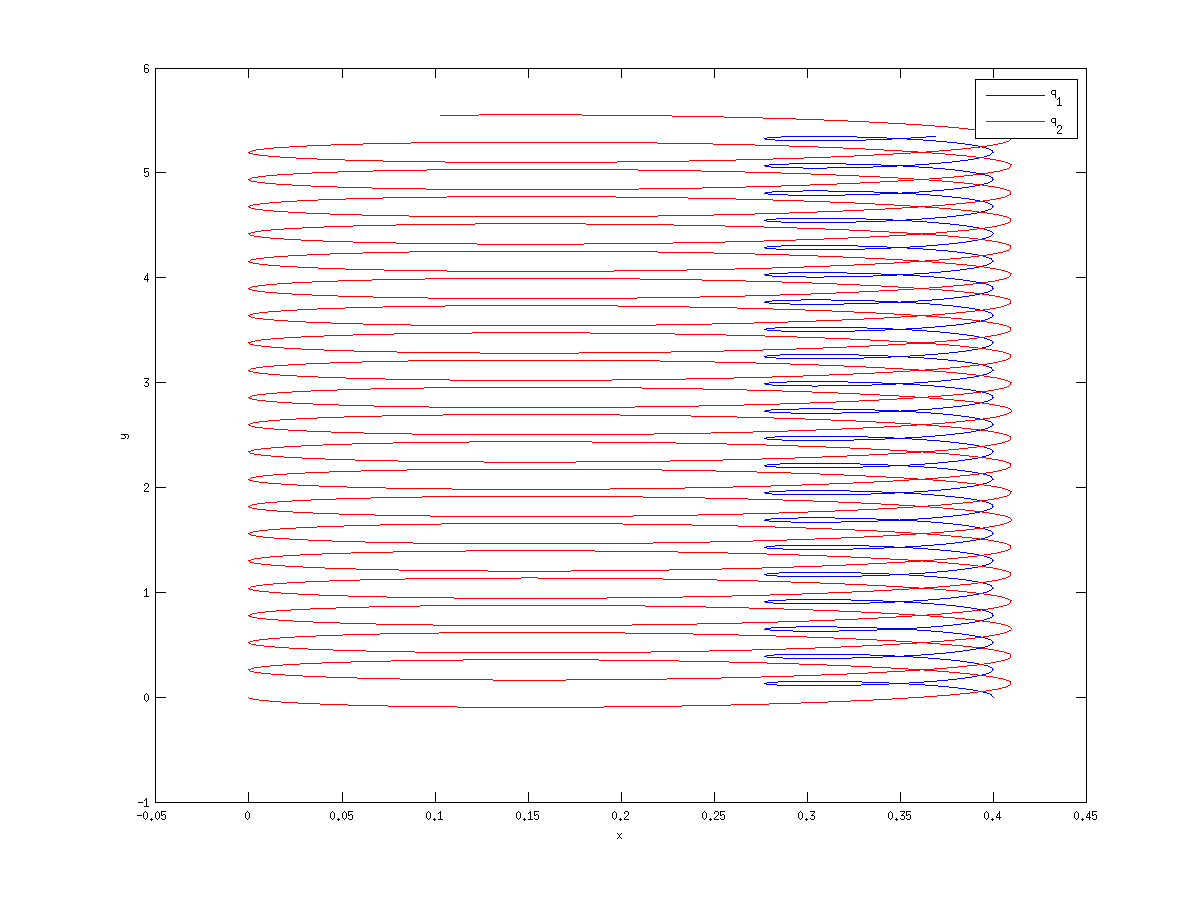
\includegraphics[width=\textwidth]{images/Q2_symplectique2_q.png}
    \caption{$q$ pour symplectique2}
    \label{fig:q2_symplectique2_q}
  \end{subfigure}%
  ~
  %(or a blank line to force the subfigure onto a new line)
  \begin{subfigure}[b]{0.3\textwidth}
    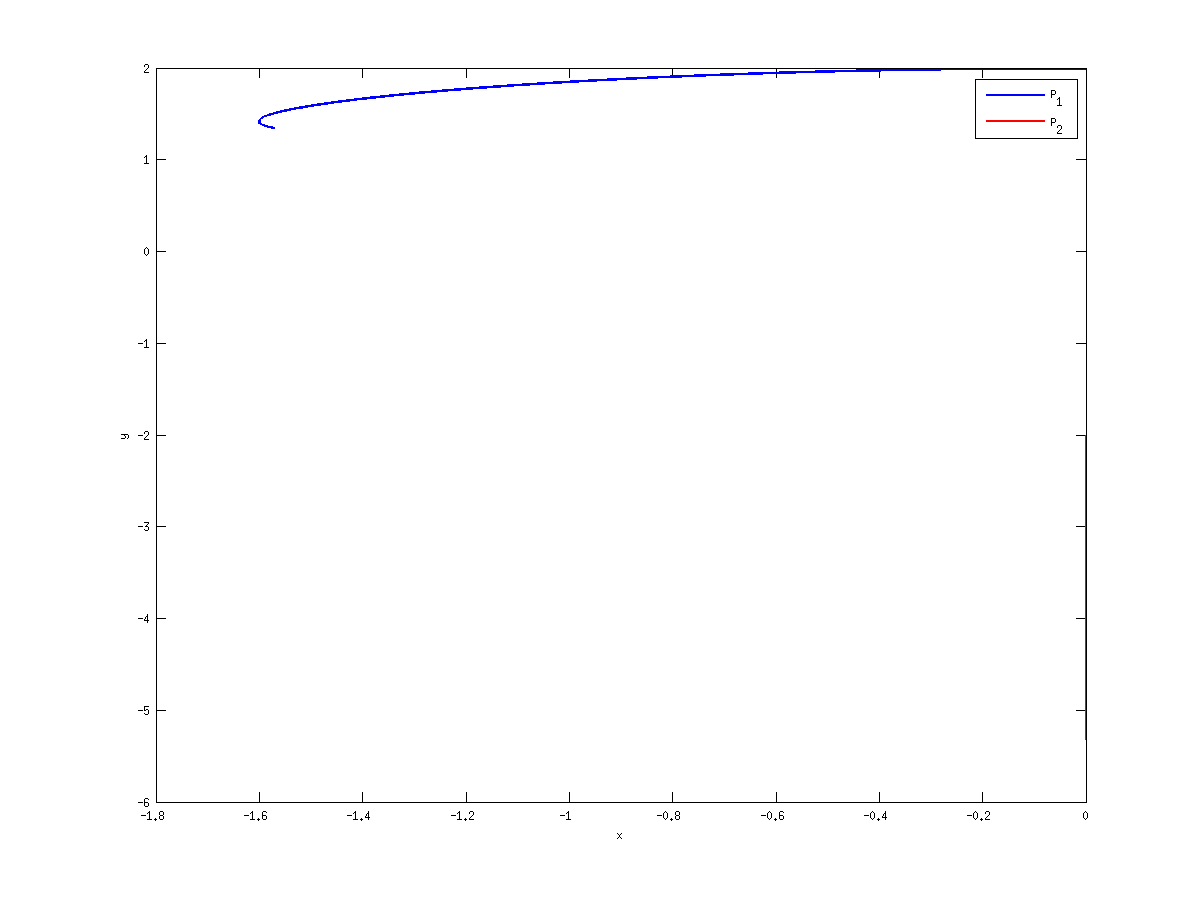
\includegraphics[width=\textwidth]{images/Q2_symplectique2_p.png}
    \caption{$p$ pour symplectique2}
    \label{fig:q2_symplectique2_p}
  \end{subfigure}
  ~
  \begin{subfigure}[b]{0.3\textwidth}
    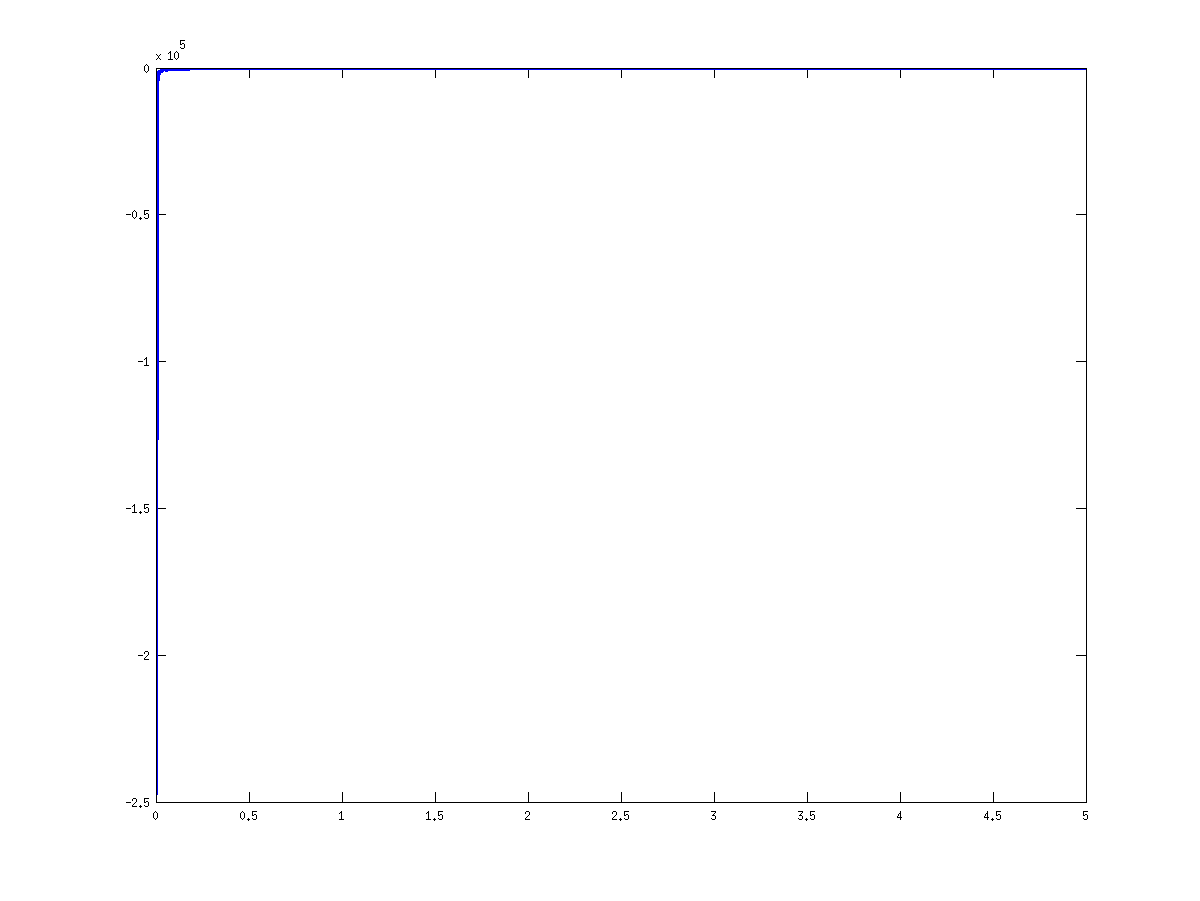
\includegraphics[width=\textwidth]{images/Q2_symplectique2_H.png}
    \caption{$\Ha$ pour symplectique2}
    \label{fig:q2_symplectique2_H}
  \end{subfigure}
  \caption{Résultats pour la question 2}\label{fig:q2}
\end{figure}
